\chapter{Introduction}
\label{chap:intro}

\section*{Cyber-physical systems}

The design of complex cyber-physical systems is an interdisciplinary process. From an engineering point of view, defining the requirements, designing sufficiently reliable components, dealing with scalability issues, employing testing processes that result in high test coverage, verifying safety critical components, and maintainability issues are all present at the same time. Systems engineering focuses on how to design and manage such systems. \cite{randomwikipedialink1} \cite{randomwikipedialink2}

\section*{Safety Critical System}

Safety-critical systems are those systems whose failure could result in loss of life, significant property damage, or damage to the environment. There are many well known examples in application areas such as medical devices, aircraft flight control, weapons, and nuclear systems. Many modem information systems are becoming safety-critical in a general sense because financial loss and even loss of life can result from their failure. Future safety-critical systems will be more common and more powerful. From a software perspective, developing safety critical systems in the numbers required and with adequate dependability is going to require significant advances in areas such as specification, architecture, verification, and process. The very visible problems that have arisen in the area of information-system security suggests that security is a major challenge also. \cite{safetycritical}

\section*{Verification}

As modern society is becoming more and more dependent on cyber-physical systems, the need for faultlessly working hardware and software increases. Validation and verification methodologies have been present in the development processes of such systems for a long time \citep{ieee1012}, but faster and more reliable approaches are needed. Validation checks that the requirements specified for the software meet the needs of the user -- as such, validation usually can be aided, but can’t entirely be done by software. The point of verification is to check whether the specified requirements are met. Methods for verification can be divided into two groups: design time verification and runtime verification.

\section*{Design time verification}

In the traditional software development methods, the verification process is in the design time. This means after the composition of system elements, we verify it's compliance with the specification. One example for this is the formal verification, where we want to proof the match in the behavior of the finished system with the specifications written in mathematically proofed formalism.

\section*{Runtime verification}

Runtime verification is based on the inspection of the running software. We watch the behavior of the system, and conforming it to the specification. This has an advantage of detecting non specified behavior after deployment. Runtime and design time verification aren't exclusive, instead of they can support a more robust system verification process. The motive of using runtime verification is the difficulty of designing highly safety systems. These systems are getting bigger in complexity, and traditional methods cannot verify it, or the resource need of a verification of this scale cannot be realized.

\section*{V-Model}

A concept of operations is one of the initial stages in a system life cycle based on the “Vee” diagram, illustrated in \cref{fig:intro:vmodel}.

\begin{figure}[h]
	\centering
	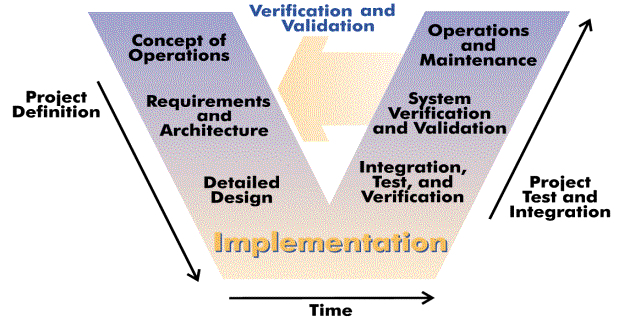
\includegraphics[width=0.8\linewidth]{include/figures/chapter_1/VModel}
	\caption{The traditional V model \cite{vmodel}}
	\label{fig:intro:vmodel}
\end{figure}

\cref{fig:intro:vmodel} shows the stages of building a system, with a symbolic “V” showing the progression from the top of the left leg of the ``V'' down to the base, across the base, and up the right leg. The project definition stages down the left side begin with development of a Concept of Operations, continue with Requirements and Architecture, and Detailed Design. The Implementation stage is shown across the base of the ``V'', with an arrow labeled ``Time'' pointing right to left across the bottom of the ``V''. The right leg shows the testing and implementation stages of a system, with an upward-pointing arrow showing the progression from the base up the leg. \cite{vmodel}

The V-Model is the basic scheme of a software development. In the left leg, we proceed down by decomposing the specifications into architecture level design, and the architecture design into component level designs. Every level of decomposition have it's own specifications. After the implementation process, we verify every levels of decompositions behavior with it's specification.

\section*{Hierarchical runtime verification}

A hierarchical runtime verification is based on the communication of runtime monitors with a higher level logic instead of a one time verification in design time. By using the V-Model, the right legs verification steps can be replaces with its runtime verification counterpart (\cref{fig:intro:rvmodel}).
These replaced elements are:
\begin{itemize}
	\item Component monitors which are the smallest, can be implemented into embedded devices.
	\item Architecture monitors which are verifying the interoperation of components.
	\item High level logic is a central element for reacting to the states of the monitors.
\end{itemize}

\begin{figure}[h]
	\centering
	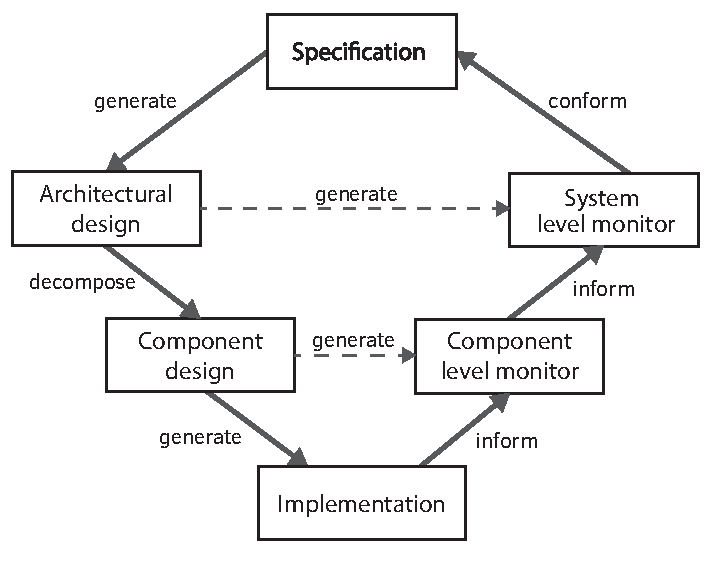
\includegraphics[width=0.8\linewidth]{include/figures/chapter_1/rv_vmodel}
	\caption{Hierarchical verification based on the V-Model}
	\label{fig:intro:rvmodel}
\end{figure}

\section*{Model driven software development}

Model driven software development (MDSD) emphasizes problem solving by the development and maintenance of models describing the system being designed. MDSD heavily relies on automated code and documentation generation based on the models of components or the overall model of the system. 

Modeling has the advantage of introducing abstractions, thus reducing the complexity of the development process. The dynamic code generation guarantees that the code will inherit the properties that can be directly derived from the model, while reducing the costs by eliminating unnecessary round-trip engineering. The generation of documentation also results in an always up-to-date description of the components, stored together with the requirements and the model. Furthermore, model based approaches have the advantage of easier testability, or if the model is formal enough they can make verification possible.

Formal verification is especially important for the development of safety critical systems (e.g.: space and flight technologies), making MDSD notably widespread in these areas.

Various methods and tools are available for the generation of test cases and monitoring components from models, as well as for formally verifying certain properties. These tools usually support a few modeling formalism of their target domain.

MDSD is usually accompanied by the Y model -- a software life cycle model for component based systems \citep{ymodel}.

\section*{Y model} % <3

\begin{figure}[h]
	\centering
	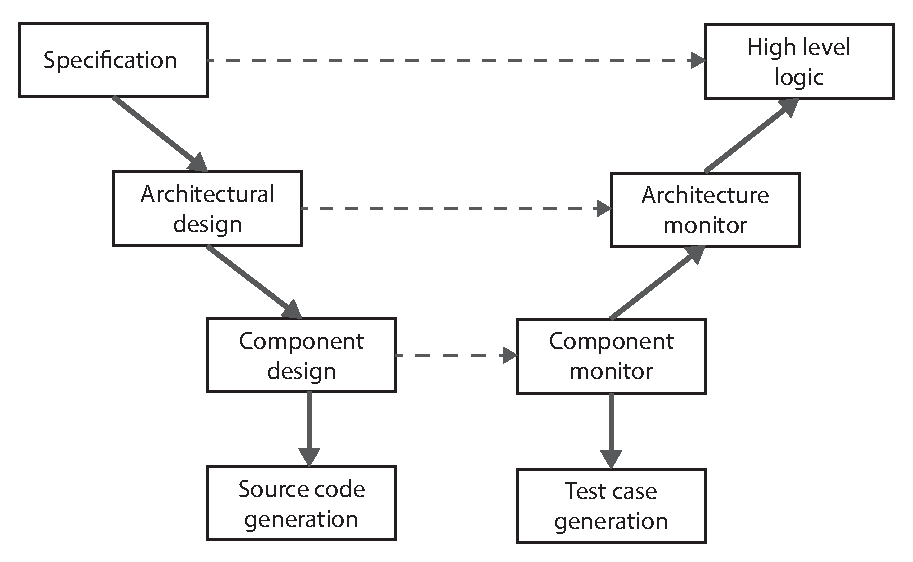
\includegraphics[width=0.8\linewidth]{include/figures/chapter_1/YModel}
	\caption{The Y model}
	\label{fig:intro:vmodel}
\end{figure}

The Y model \citep{ymodel} is an extension of the V model (which is in turn an extension of the waterfall model) \citep{randomwikipedialink3}, by using code and test case generation. Much like the V model, the development process is partitioned vertically. Each level contains a model that is transformed to a verification model, on which formal methods can be applied. The results of the verification process can be traced back to the original models making iterative improvement possible. The top level is for high level system models, while the second level contains architectural models, and the third one is for component based models. This provides input for the last step, source code and configuration generation for the individual components. Test cases are paired with the source code and can be generated from the component verification models.

\section*{Modeling approaches}

MDSD methods require modeling languages to describe the behavior of systems and components. Engineering practices developed a wide range of such languages over the years to support fast paced product development. This allows the use of domain specific languages, which leads to a shorter modeling process but challenges formal verification software, as their input is usually stricter and in a more general format. The result is the need for complex model transformations before the verification can begin, which can lead to higher development costs, or -- if the transformation contains errors -- even faulty behaviour.\\
As a result, standardized modeling languages were developed like the UML (Unified Modeling Language \citep{uml}) and SysML (Systems Modeling Language \citep{sysml}) languages.

\subsection*{CEP}

\begin{figure}[h]
	\centering
	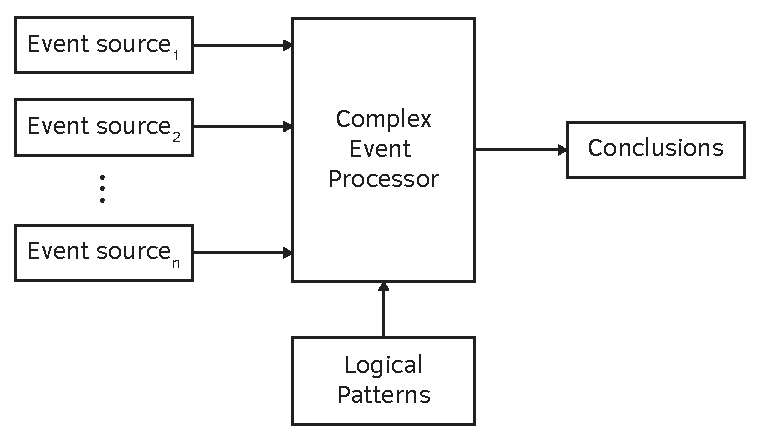
\includegraphics[width=0.8\linewidth]{include/figures/chapter_1/CEP}
	\caption{CEP overview}
	\label{fig:intro:vmodel}
\end{figure}

Complex event processing is a method of tracking and analysis streams of information and deriving conclusions. In a complex event processing environment, there can be multiple event sources, and with logical patterns given by a formalism, we can find patterns in the incoming stream, e.g. events followed by another events in some sequence: \citep{epbas}

\subsection*{Finite automaton}

Modelling a system with finite state space is often done by using finite automata -- also known as finite state machines. A finite automaton accepts a (finite) list of symbols and produces a computation of the automaton for each input list.
Although finite automata can be easily visualized, this formalism describes a simple, flat transition system and lacks the support for higher level concepts. The development of finite automata models  are supported by many tools (e.g.: Finite State Machine Designer \citep{yakindu}).

\subsection*{Statechart}

Statecharts, also known as state machines are an extension of finite automata. There are multiple available syntaxes for statecharts (e.g. the one defined by UML \citep{stcuml}). The higher level concepts that were introduced include variables, actions, and hierarchically nested states. Event-driven execution is also possible by using signals as the triggers of transitions. Available variable types heavily depend on the concrete semantics of the chosen statechart language. Actions can usually be variable assignments, signal raises, or the setting of timers. Hierarchy lets users organize system descriptions using a top-down approach. Support for hierarchy is introduced via nested states and parallel regions. States can also have entry and exit actions, which allows the description of common functionality in parent states \citep{stcmove}.\\
Statecharts are usually created by tools that support the graphical design of the model (e.g.: Yakindu, an Eclipse based editor).


\subsection*{Sequence Chart}

The formalism of message sequence charts (MSC) describes the communication between components -- the order in which messages can occur \citep{msc} \citep{msc2}. The message interchange is usually represented by a graphical model. These charts can be used for high level specification, design, trace based testing, or documentation. A collection of possible sequence charts can also describe a complete communication protocol between components. UML sequence diagrams were inspired by MSCs, but their semantics differ regarding some of the basic elements of the language such as lifelines and arrows \citep{mscuml}.

\section*{Contributions}

Our goal was to provide runtime verification methods for all levels of a complex cyber-physical system. These methods should rely on modelling methods already being used be engineers to minimize the steepness of the learning curve and allow quick and efficient development. The result is a hierarchical runtime verification framework which can enable verification on two levels. The framework is capable of:
\begin{itemize}
  \item component level verification, supported by the generation of monitors from statecharts
  \item system level verification, that can be done by a complex event processing system
  \item monitors can generate messages indicating erroneous operation of the monitored components
  \item the complex event processing system can use the monitors' messages
\end{itemize}
\begin{figure}[h]
	\centering
	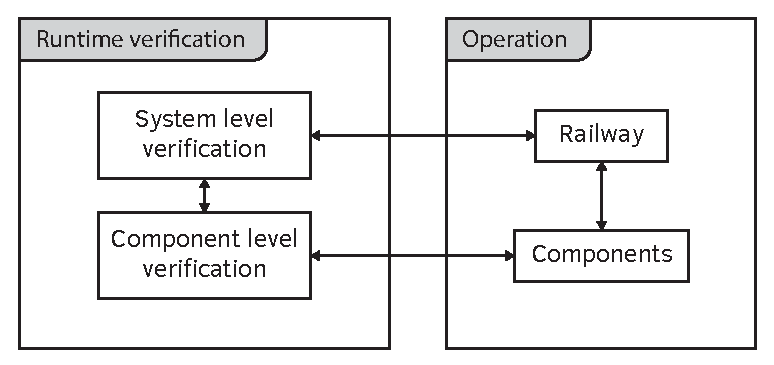
\includegraphics[width=0.5\linewidth]{include/figures/chapter_1/rv_concept}
	\caption{Overview of the hierarchical runtime verification system}
	\label{fig:case_study:fov}
\end{figure}
Additionally, the statechart language developed extends the usual statechart formalism by adding support for statechart templates. This enables users to easily describe systems with homogeneous components. The models can also be mapped to a formally verifiable transition system.
\\\textbf{TODO}\\
Automata generalas?
CEP egyebek?

This hierarchical approach to runtime verification results in safer systems with more dependable monitoring components.